% ============================================================
%  Between-epoch carry: arrowhead admissibility and the DD
%  cycle basis
%
%  Companion to the Network-mode section.  Where sec:net-schur
%  STATES the arrowhead reduction, this document develops its
%  consequences: which folds an arrowhead system admits and
%  where, why the carried time-linked quantity must be the
%  double-differenced cycle basis (chords), and the Woodbury
%  algebra that folds it.  Closes with a fully numerical
%  minimum-parameter example (2 receivers x 2 satellites, one
%  chord) carried end to end.
%
%  Sources: filter/NetworkNormalEquations (addStationPrior,
%  addSharedInfo, foldReducedSumZeroGauges, foldReducedDdPriors,
%  ddPriorPosteriorMean/Covariance, ddPriorInnovation),
%  filter/NetworkZStore (ArcKey / ZComponent cycle algebra),
%  filter/NetworkInvariantCarryDriver (the per-epoch reconcile),
%  filter/NetworkEstimator (setDdPriors, the datum seam).
%
%  Every number in the worked example is exact and was checked
%  against a dense stacked solve of the same system.
%
%  Note on citations: the two generalised-filter papers this
%  material rests on (Teunissen, Khodabandeh & Psychas 2021;
%  Hou & Zhang 2025) are cited in prose with journal, volume and
%  article number rather than through references.bib, which does
%  not carry them.
%
%  Standalone-compilable subfile (shares gnssreport.sty via the
%  subfiles package).  Wired into the combined volume after
%  \subfile{network_example} in main.tex.
% ============================================================
\documentclass[main.tex]{subfiles}
\begin{document}
\ifSubfilesClassLoaded{\begin{center}\small\itshape Part of the GnssProcessor Mathematical Reference \textbullet\ \today\end{center}}{}

\section{Between-epoch carry: arrowhead admissibility and the DD cycle basis}
\label{sec:net-carry}

% Shared with the Network-mode document; \providecommand so the two
% subfiles can be combined in either order without a redefinition error.
\providecommand{\Nss}{\bm{N}_{ss}}            % shared (satellite) normal block
\providecommand{\Nrr}{\bm{N}_{rr}}            % per-station local normal block
\providecommand{\Nsr}{\bm{N}_{sr}}            % shared<->local cross block
\providecommand{\redNss}{\tilde{\bm{N}}_{ss}} % Schur-reduced shared normals
\providecommand{\redus}{\tilde{\bm{u}}_s}     % Schur-reduced shared RHS
\providecommand{\xshared}{\bm{x}_s}           % shared satellite-parameter estimate
\providecommand{\xlocal}[1]{\bm{x}_{#1}}      % station r's private nuisance block
% Doc-local, deliberately non-trivial names (see the subfiles macro-collision note).
\providecommand{\Czmat}{\bm{C}_L}             % cycle-coefficient matrix on local columns
\providecommand{\Czrx}[1]{\bm{C}_{L,#1}}      % ... restricted to one station's columns
\providecommand{\Pzmat}{\bm{P}^{z}}           % carried DD prior covariance
% Pzmat already carries a superscript: these avoid a double-superscript clash.
\providecommand{\Pzinv}{(\bm{P}^{z})^{-1}}
\providecommand{\Pzpost}{\bm{P}^{z+}}
\providecommand{\Pzprior}{\bm{P}^{z,\mathrm{prior}}}
\providecommand{\Bfold}{\bm{B}}               % C_L Nrr^{-1} C_L^T
\providecommand{\Gfold}{\bm{G}}               % Nsr Nrr^{-1} C_L^T
\providecommand{\Mfold}{\bm{M}}               % (P^z + B)^{-1}
\providecommand{\zfreev}{\bm{z}_{\mathrm{free}}}
\providecommand{\Sigss}{\bm{\Sigma}_{ss}}     % datum-as-known shared covariance
\providecommand{\arcset}{\mathcal{E}}         % arc set of the observation graph

The Network-mode document establishes the arrowhead normal-equation
topology and its exact Schur reduction
(\dcref{sec:net-schur}{the per-station Schur reduction section of the
Network-mode document}), and the worked estimability example establishes
the minimum-constraint datum
(\dcref{sec:net-example}{the two-receiver estimability example}).  This
document covers the step between them: \emph{how information from
outside the current epoch enters an arrowhead system}.

The structure of the problem sets the requirements.  A network producer
that solves each epoch independently discards what it has learned about
the carrier-phase ambiguities, the only constant quantities in the
problem.  A producer that carries them without care destroys either the
sparsity that keeps the solve affordable or the datum invariance that
gives the product its meaning.  The design has three parts, developed in
order:

\begin{enumerate}[leftmargin=*, itemsep=1pt]
\item An arrowhead system admits exactly \emph{three} kinds of
      information fold.  The columns the new information touches
      determine which one applies; its physical meaning does not
      (\Cref{sec:net-carry-doors}).
\item The carried quantity must therefore be gauge-free.  The natural
      gauge-free basis of the ambiguity block is the \emph{cycle space}
      of the receiver--satellite observation graph: the double
      differences indexed by the spanning tree's \emph{chords}
      (\Cref{sec:net-carry-cycles}).
\item Carrying that basis costs one bounded Woodbury correction per
      connected component, with closed forms for the posterior and for
      an exact innovation test (\Cref{sec:net-carry-fold}).
\end{enumerate}

\Cref{sec:net-carry-example} then carries a two-receiver,
two-satellite network, the smallest network whose observation graph
has a cycle, through every step with exact arithmetic.

The golden configurations do not arm the invariant DD carry developed
here (\texttt{network.carry\_invariant} is false in both); they carry
the float ambiguity vehicle instead
(\dcref{sec:net-vehicle}{the float-ambiguity-vehicle section}).  The
door analysis of \Cref{sec:net-carry-doors} still governs where that
vehicle's folds enter.  The shared-border carry takes door~1, and the
vehicle's per-station block, with its regression on the shared border,
enters before the reduction as whitened rows of that station's own
design (\texttt{CouplingRowBuilder::buildLocalBlock},
\texttt{filter/NetworkCoupling}), so it touches only that station's
blocks and is bound by door~2's ordering constraint.  No golden fold
takes door~3.

\begin{remark}[Theoretical footing]
Time-linking a \emph{selected} set of linear functions $\bm{z} =
\bm{F}^\Tr\bm{x}$ while re-estimating the remainder fresh each epoch is
the generalised Kalman filter of Teunissen, Khodabandeh \& Psychas
(\emph{J.\ Geod.}\ 95:108, 2021) and the generalised least-squares
filter of Hou \& Zhang (\emph{J.\ Geod.}\ 99:3, 2025).  Both leave open
the construction of the transition $\bm{\Phi}^z$ of the linked functions
across a \emph{changing} linked set.  Choosing $\bm{z}$ as the cycle
basis closes that gap: every basis change the graph can force is then a
unimodular integer matrix (\Cref{sec:net-carry-cycles}).  The
spanning-tree S-basis itself is due to \textcite{deJonge1998processing},
who selects it once and never re-selects it.  The construction here
extends it to a basis that changes from epoch to epoch.
\end{remark}

% ------------------------------------------------------------------
\subsection{Three doors into an arrowhead system}
\label{sec:net-carry-doors}

The epoch's system has the structure of
\dcref{sec:net-schur}{the Schur reduction section}: a shared satellite
border $\xshared$, one private block $\xlocal{\rx}$ per station, and
zero station--station coupling.  Consider a Gaussian prior
$\bm{z}\sim N(\hat{\bm{z}}, \Pzmat)$ on a linear function
$\bm{z} = \bm{C}\bm{x}$ of the epoch's parameters.  In information form
it is the increment $\bm{C}^\Tr\Pzinv\bm{C}$ to the normal matrix
and $\bm{C}^\Tr\Pzinv\hat{\bm{z}}$ to the right-hand side.  The block in
which that increment lands determines how it can be folded.

\paragraph{Door 1: the shared border.}
If $\bm{C}$ touches only shared columns, the increment lands entirely in
$\Nss$.  Such a fold is \emph{reduction-preserving}:

\begin{samepage}
\begin{quote}
\textbf{Lemma.} For any symmetric $\Delta\bm{N}$ and any $\Delta\bm{u}$
on the shared border,
\[
  \widetilde{\left(\Nss + \Delta\bm{N}\right)} = \redNss + \Delta\bm{N},
  \qquad
  \widetilde{\left(\bm{u}_s + \Delta\bm{u}\right)} = \redus + \Delta\bm{u}.
\]
\emph{Proof.} The Schur subtrahend
$\sum_\rx \Nsr^{\,\rx}(\Nrr^{\,\rx})^{-1}\Nsr^{\,\rx\Tr}$ is a function
of $\Nsr$ and $\Nrr$ only; $\Nss$ enters
\dcref{eq:net-schur-N}{the reduced-normals equation} additively.
\hfill$\square$
\end{quote}
\end{samepage}

A border prior may therefore be folded \emph{before or after} the
reduction with identical results.  The between-epoch carry of the
satellite clock and biases costs no second Schur pass even when it is
applied late, for example between the null-space rank gate and the
solve.  \texttt{addSharedInfo} (\texttt{filter/NetworkNormalEquations})
uses this: when a reduction is already cached, it folds the delta in
place and leaves the cache current.  The dense form of the same carry
(\texttt{addSharedPriorDense}, \texttt{NetworkEstimator}) takes a
\emph{covariance} rather than an information matrix.  A carried key
absent from the current epoch's layout must be \emph{marginalised}, a
row and column deletion on $\Pzmat$; deleting the same rows of $\Pzinv$
would instead \emph{condition} on the departed key and bias every
surviving parameter.

\paragraph{Door 2: one station's own columns, before the reduction.}
If $\bm{C}$ touches only station $\rx$'s local columns, the increment
lands in $\Nrr^{\,\rx}$.  For a diagonal prior on columns
$c \in \mathcal{C}$ with information weights $\Lambda_c \ge 0$ and
information right-hand sides $\eta_c$,
\begin{equation}
\Nrr^{\,\rx} \mathrel{+}= \sum_{c\in\mathcal{C}} \Lambda_c\,
   \bm{e}_c\bm{e}_c^\Tr,
\qquad
\bm{u}_r^{\,\rx} \mathrel{+}= \sum_{c\in\mathcal{C}} \eta_c\,\bm{e}_c ,
\label{eq:carry-localprior}
\end{equation}
which the implementation applies as a sequence of rank-one updates of
the \emph{cached} $\mathrm{LDL}^\Tr$ factor
(\texttt{addStationPrior}).  The raw $\Nrr$ is never stored or
re-factorised, and a positive $\Lambda_c$ keeps the factor
positive-definite by construction (a zero weight skips the factor
update and still adds its right-hand-side increment).  Unlike door~1,
this fold is \emph{not} reduction-preserving: it changes $\Nrr$, hence
the Schur subtrahend, hence $\redNss$.  It must be applied
\emph{before} the reduction; there is no post-reduce fast path.  It is
cheap for two reasons: it is orthogonal to every other station (the
arrowhead has no station--station block to disturb), and it conditions
only $\xlocal{\rx}$.

The two doors have opposite ordering constraints: door~1 may be late,
door~2 must be early.  The asymmetry follows directly from
\dcref{eq:net-schur-N}{the reduced-normals equation}.

\paragraph{Door 3: local columns across several stations.}
If $\bm{C}$ touches local columns of two or more stations, the
information increment $\bm{C}^\Tr\Pzinv\bm{C}$ has a nonzero
$(\rx,\rx')$ block.  It is representable neither as a border increment
nor as a per-station one.  Folding it into the unreduced system
\emph{destroys the arrowhead}: it fills in the station--station zeros
that make the marginalisation exact and cheap.

This is the case that matters in practice.  The only ambiguity
combinations worth carrying are between-station ones, because a single
station's ambiguity is not estimable on its own
(\dcref{sec:net-example-phase}{the phase part of the two-receiver
example}).  Such a prior is folded \emph{after} the reduction, by
Woodbury through the block-diagonal local normals, using the
per-station factors the reduction has already computed and left
intact.  \Cref{sec:net-carry-fold} gives the algebra; the rest of this
subsection records the two hazards it creates.

\begin{remark}[Post-reduce folds do not compose]
Two door-3 folds applied to the same reduced system are each derived
against the \emph{pristine} $\Nrr$.  Composing them over coupled local
columns is therefore inexact: neither fold sees the other's
augmentation of $\Nrr$, so the composition drops the cross term
$\Czmat\Nrr^{-1}\bm{C}_{L,\text{other}}^{\Tr}$ of the joint middle
inverse without any signal.  The implementation enforces the exclusion:
the sum-to-zero ensemble phase gauge (\texttt{foldReducedSumZeroGauges})
and the carried DD priors (\texttt{foldReducedDdPriors}) are mutually
exclusive, and \texttt{NetworkEstimator::solve} throws if both are set.
Under the invariant carry the phase datum is realised instead through
door~2, by the pre-reduce tree pins.  These compose \emph{exactly} with a
post-reduce door~3 fold, because the fold then reads an already-pinned
factor.

The same truncation applies between DD blocks.
\texttt{foldReducedDdPriors} folds one block per connected component of
one (constellation, signal) group, each against the unmodified
per-station factors, so the result is exact only when no station is touched by two blocks.  A
station tracking two signals sits in two blocks, and the fold then
makes the block-Jacobi approximation of dropping the cross terms between
them.
\end{remark}

\begin{remark}[A door-3 fold cannot repair a rank deficiency]
Let $\delta\xshared$ span a null direction of $\redNss$, with the
matching local response $\delta\xlocal{\rx} =
-(\Nrr^{\,\rx})^{-1}\Nsr^{\,\rx\Tr}\delta\xshared$.  If the carried
function is estimable, $\bm{z} = \Czmat\bm{x}_L$ is invariant along that
direction, so $\Czmat\,\delta\bm{x}_L = -\Gfold^\Tr\delta\xshared = 0$
with $\Gfold$ as defined in \Cref{eq:carry-fold-blocks}.  Every column
of $\Gfold$ is therefore orthogonal to the null space, the rank-$K$
update $\Gfold\Mfold\Gfold^\Tr$ adds nothing along it, and the declared
S-basis dimension the rank gate tests is unchanged by the carry.  A
carry that changed it would be carrying a gauge rather than
information.
\end{remark}

% ------------------------------------------------------------------
\subsection{The observation graph and its cycle space}
\label{sec:net-carry-cycles}

Door~3 admits only gauge-free functions, and the carried basis is
chosen accordingly.  The graph structure determines that choice; no
numerical criterion enters.

\paragraph{The graph.}
For a constellation $g$ and a signal $\sigl$, let $G_{g,\sigl} = (V,
\arcset)$ be the graph whose vertices $V = \rxset \cup \satset{g}$ are
the receivers and the satellites, and whose \emph{arcs} are the
receiver--satellite pairs carrying an ambiguity this epoch:
$(\rx,\sat) \in \arcset$ iff station $\rx$ tracks satellite $\sat$ on
signal $\sigl$.  There is at most one arc per pair, so an unordered
vertex pair is a unique arc identity (\texttt{ArcKey},
\texttt{filter/NetworkZStore}).  The graph is \emph{bipartite} by
construction: no arc joins two receivers or two satellites.

\paragraph{Trees and chords.}
A connected component with $n_c$ receivers, $m_c$ satellites and
$|\arcset_c|$ arcs has a spanning tree of $n_c + m_c - 1$ edges.  The
remaining
\begin{equation}
K_c \;=\; |\arcset_c| \;-\; (n_c + m_c - 1)
\label{eq:carry-chordcount}
\end{equation}
arcs are the \emph{chords}.  Adding a chord to the tree closes exactly
one cycle, its \emph{fundamental cycle}: the chord plus the unique
tree path joining its endpoints.  The $K_c$ fundamental cycles are a
basis of the component's cycle space.  \Cref{eq:carry-chordcount} is
the first Betti number of the component.  It is the exact number of
independent double differences the component supports, and it is a
property of the \emph{graph}, independent of the estimator.

\paragraph{The carried functions.}
The graph is bipartite, so every cycle alternates
receiver--satellite--receiver--satellite, has even length, and admits
an alternating signing of its arcs.  For chord $c$ with fundamental
cycle $\mathcal{C}_c$, define
\begin{equation}
z_c \;=\; \sum_{(\rx,\sat)\,\in\,\mathcal{C}_c}
          \sigma_{(\rx,\sat)}\, N^{\sat}_{\rx,\sigl},
\qquad \sigma_{(\rx,\sat)} = \pm 1 \ \text{alternating},
\label{eq:carry-cycle-sum}
\end{equation}
which for the shortest cycle (length four) is a plain double difference
$N^{\sat_1}_{\rx_1} - N^{\sat_1}_{\rx_2} + N^{\sat_2}_{\rx_2} -
N^{\sat_2}_{\rx_1}$, and for a longer fundamental cycle is a
higher-order alternating difference on six or more columns.

\begin{samepage}
\begin{quote}
\textbf{Proposition (gauge-freeness).} $z_c$ is invariant under both
ambiguity gauges of the network model: the receiver shift
$N^{\sat}_{\rx}\mapsto N^{\sat}_{\rx} - d_{\rx}$ for all $\sat$, and the
satellite shift $N^{\sat}_{\rx}\mapsto N^{\sat}_{\rx} - c^{\sat}$ for
all $\rx$.

\emph{Proof.} A cycle visits each of its vertices exactly once, and each
visited vertex is incident to exactly \emph{two} arcs of the cycle,
which by the alternating signing carry opposite signs.  A shift attached
to that vertex ($d_\rx$ at a receiver, $c^{\sat}$ at a satellite)
therefore contributes $(+1)\delta + (-1)\delta = 0$ to
\Cref{eq:carry-cycle-sum}.  Summing over vertices gives invariance.
\hfill$\square$
\end{quote}
\end{samepage}

Hence $z_c$ touches no shared column: the receiver and satellite phase
biases cancel analytically rather than numerically.  Three consequences
follow, and together they make the cycle basis the carried object:

\begin{itemize}[leftmargin=*, itemsep=1pt]
\item \textbf{Estimable in every S-system.}  $z_c$ is invariant under
      the datum, so it may be compared across epochs whose datum
      differs and graded without an S-transform
      (\dcref{sec:net-sbasis}{the minimum-constraint datum section}).
\item \textbf{Integer, and constant between slips.}  $z_c$ is an
      integer combination of integer ambiguities, and its process noise
      is $q_z = 0$ in the absence of a cycle slip.  It is the \emph{only}
      part of the ambiguity block for which a zero-$q$ time link is
      physically correct.
\item \textbf{Basis changes are unimodular.}  Two spanning trees of the
      same arc set give cycle bases related by an integer matrix
      $\bm{T}$ with $\det\bm{T} = \pm1$, so $\bm{z}' = \bm{T}\bm{z}$,
      $\Pzmat{}' = \bm{T}\Pzmat\bm{T}^\Tr$ is an \emph{exact} change of
      basis with no information loss.  Basis churn defeats any carry of
      the raw ambiguities, whose individual values depend on the datum;
      in the cycle basis it has no effect by construction.
\end{itemize}

\paragraph{Graph events are exact operations.}
Every way the graph can change between epochs maps to an exact
operation on the carried $(\hat{\bm{z}}, \Pzmat)$
(\texttt{ZComponent}, \texttt{filter/NetworkZStore}):

\begin{center}\small
\begin{tabular}{@{}p{0.36\linewidth}p{0.58\linewidth}@{}}
\toprule
Graph event & Operation on the store \\
\midrule
Chord dies (arc lost) &
  Drop that row and column of $\Pzmat$, pure marginalisation \\
Chord born (arc closes a new cycle) &
  Append an entry initialised by tap-off
  $\hat z_{\text{new}} = \bm{f}^\Tr\hat{\bm{x}}$ with its conditional
  variance and cross-covariances \\
Leaf growth (arc brings in a new vertex) &
  Extends the tree, closes no cycle, touches no $z$ \\
Tree edge dies &
  Pivot a covering chord into the tree
  ($\bm{z}'=\bm{T}\bm{z}$, $\bm{T}$ unimodular), then kill the arc as a
  chord.  An uncovered tree edge is a cut edge: its death splits the
  component, which merely re-partitions existing blocks \\
Components merge &
  Union the two blocks block-diagonally (they were independent),
  promote one bridge arc to the tree, tap off any surplus bridges \\
\bottomrule
\end{tabular}
\end{center}

The producer does not apply these as a sequence of events.  The
per-epoch driver (\texttt{filter/NetworkInvariantCarryDriver}) receives
the current epoch's tree/chord partition from the election and computes
the \emph{composed} transform directly.  A new chord's fundamental cycle
lies in the previous epoch's cycle space if and only if every arc of
that cycle was present last epoch; its carried mean is then
$\hat z^{\text{new}}_c = \sum_j w_j\,\hat z^{\text{old}}_j$, with
$w_j$ the incidence of old chord $j$'s arc in the new cycle.  Assembling
$\bm{W}$ over the contributing components gives
$\hat{\bm{z}}^{\text{prior}} = \bm{W}\hat{\bm{z}}^{\text{old}}$ and
$\Pzprior = \bm{W}\Pzmat\bm{W}^\Tr$.  A dead chord's column of $\bm{W}$
is zero (marginalisation).  Merges and splits follow from the
contributor gather with no special case.

A chord whose cycle uses a newborn arc is \emph{fresh}.  The driver
gives it a finite diffuse prior (variance \texttt{fresh\_prior\_var},
default 1.0e6 in state units squared) rather than the exact
zero-information tap-off of the table.  Its posterior is therefore the
data-only tap-off up to a term of the order of the ratio of the data
variance to \texttt{fresh\_prior\_var}.  An arc
flagged as slipped this epoch counts as absent from the previous arc set,
so every chord whose cycle uses it is also born fresh (for a two-band
pair group under the lane shape, the driver takes the union of the
band-1 and band-2 slip flags).  The production caller passes only arcs
that resolve to an estimator column; a carried chord whose cycle has an
unresolvable arc this epoch is dropped from the carry and re-tapped when
the arc returns.

\begin{remark}[Why the tree must avoid slipped arcs]
A slip on a \emph{chord} costs exactly one carried DD.  A slip on a
\emph{tree edge} corrupts every fundamental cycle routed through it.
With \texttt{network.phase\_datum\_eq34\_slip\_aware\_election} armed
(default off), the election therefore keeps slipped arcs out of the
tree wherever the graph allows it.  The argument is structural and
independent of any detector threshold.
\end{remark}

% ------------------------------------------------------------------
\subsection{Folding the carried double differences}
\label{sec:net-carry-fold}

Let one connected component carry $K$ double differences with prior mean
$\hat{\bm{z}}$ and covariance $\Pzmat$, expressed as
$\bm{z} = \Czmat\bm{x}_L$ where $\Czmat$ is the $K \times n_L$ signed
incidence matrix of \Cref{eq:carry-cycle-sum} over the epoch's local
ambiguity columns, and $\Czrx{\rx}$ is its restriction to station
$\rx$.  This is a door-3 fold.  Woodbury through the block-diagonal
local normals gives, per component,
\begin{equation}
\Bfold = \sum_\rx \Czrx{\rx}\Nrr^{-1}\Czrx{\rx}^\Tr,
\quad
\Gfold = \sum_\rx \Nsr\Nrr^{-1}\Czrx{\rx}^\Tr,
\quad
\zfreev = \sum_\rx \Czrx{\rx}\Nrr^{-1}\bm{u}_r,
\quad
\Mfold = (\Pzmat + \Bfold)^{-1},
\label{eq:carry-fold-blocks}
\end{equation}
and the reduced system takes the rank-$K$ correction
\begin{empheq}[box=\fbox]{align}
\redNss &\mathrel{+}= \Gfold\,\Mfold\,\Gfold^\Tr,
\label{eq:carry-fold-N}\\
\redus  &\mathrel{+}= \Gfold\,\Mfold\,(\zfreev - \hat{\bm{z}}).
\label{eq:carry-fold-u}
\end{empheq}
Every ingredient of \Cref{eq:carry-fold-blocks} comes from the
\emph{cached} per-station $\mathrm{LDL}^\Tr$ factors.  No re-reduction
is needed and the factors are left unmodified.  The only new inverse is
the $K \times K$ middle matrix $\Mfold$, which is per component and
bounded in size.  Back-substitution then returns the \emph{constrained}
locals,
\begin{equation}
\xlocal{\rx} \mathrel{-}=
  \Nrr^{-1}\Czrx{\rx}^\Tr\,\Mfold\,
  \big(\zfreev - \Gfold^\Tr\xshared - \hat{\bm{z}}\big),
\label{eq:carry-fold-backsub}
\end{equation}
so the ambiguities read by the quality-control layer and by the next
epoch's tap-off are in the same frame as the fold.

\paragraph{Posterior.}
The value the store carries forward is the prior shrunk towards the
data-implied DD,
\begin{equation}
\hat{\bm{z}}^{+} = \hat{\bm{z}} + \Pzmat\,\Mfold\,\bm{v},
\qquad
\bm{v} = \zfreev - \Gfold^\Tr\xshared - \hat{\bm{z}},
\label{eq:carry-post-mean}
\end{equation}
with covariance, in the datum-as-known shared frame $\Sigss$ (the
solve's shared covariance with every datum-pinned and gauge column
treated as exact),
\begin{equation}
\Pzpost = \underbrace{\left(\Pzmat - \Pzmat\Mfold\Pzmat\right)}
             _{\text{conditional on }\xshared}
             \;+\; \left(\Pzmat\Mfold\Gfold^\Tr\right)\Sigss
                   \left(\Gfold\Mfold\Pzmat\right).
\label{eq:carry-post-cov}
\end{equation}
The first term is the posterior given the border; the second restores
the coupling through it.  $\Sigss$ is datum-constrained, but $\Pzpost$
is datum-invariant because $\bm{z}$ is estimable.
\texttt{ddPriorPosteriorMean} and \texttt{ddPriorPosteriorCovariance}
evaluate the two expressions per block from the cached fold factors.

\paragraph{Innovation.}
The same factors give an exact test of the carry against the epoch's
data (\texttt{ddPriorInnovation}).  Under the null hypothesis that the
carried DD is still valid,
\begin{equation}
\bm{v} = \zfreev - \Gfold^\Tr\xshared - \hat{\bm{z}},
\qquad
\mathrm{Cov}(\bm{v}) = \Mfold^{-1} - \Gfold^\Tr\,\Sigss\,\Gfold ,
\label{eq:carry-innov}
\end{equation}
and $|v_i|/\sqrt{\mathrm{Cov}(\bm{v})_{ii}}$ is the standardised
statistic that flags a slipped carried DD for re-tapping.  With
\texttt{network.carry\_invariant\_innov\_gate} armed (default off), the
driver flags a chord when the statistic exceeds
\texttt{network.carry\_invariant\_innov\_k} (default 4.0) times a
scale factor: 1 by default, or the LS-VCE estimate of the empirical
innovation scale when \texttt{network.carry\_invariant\_innov\_calibrate}
is armed.  The \emph{minus} sign in \Cref{eq:carry-innov} is
exact rather than a conservative approximation.  $\xshared$ is itself
influenced by the prior through \Cref{eq:carry-fold-u}, and subtracting
$\Gfold^\Tr\Sigss\Gfold$ corrects for testing the carry against a
solution the carry helped produce.  Consistency with
\Cref{eq:carry-post-mean,eq:carry-post-cov} is direct:
$\Pzmat\Mfold\,\mathrm{Cov}(\bm{v})\,\Mfold\Pzmat = \Pzmat -
\Pzpost$.

\paragraph{The hard-constraint limit.}
Setting $K=1$, $\hat z = 0$ and $\Pzmat \to \bm{0}$ turns
\Cref{eq:carry-fold-N,eq:carry-fold-u} into the rank-one fold of an
exact linear constraint $\sum_\rx z_\rx = 0$ on local columns, with
$\Mfold \to \Bfold^{-1}$.  That is the anchor-free sum-to-zero
phase-bias gauge (\texttt{foldReducedSumZeroGauges}).  The DD prior is
its soft generalisation: the two are the same object, which is why they
cannot be composed.

\paragraph{Positive-definiteness, and why it is counted.}
$\Pzmat + \Bfold$ is positive-definite in exact arithmetic, but it can
fail to be numerically.  A stiff carry ($\Pzmat$ near zero) added to an
ill-conditioned $\Bfold$ subtracts operands of similar magnitude to
reach a much smaller result.  When the screen fails, the fold is applied
\emph{inertly}, $\Mfold := \bm{0}$: the reduced system is untouched and
the posterior equals the prior.  The block keeps its slot, so the
per-block readouts stay index-aligned with the carry's block list.

The inert branch raises no error, and that makes it hazardous.  The
component's carried sub-state stops taking data, while every downstream
reading of it (its formal $\sigma$, the innovation test, any
ambiguity-resolution probe) continues to report on a quantity that is
no longer updated.  A carry can therefore diffuse for hundreds of
epochs behind clean logs.  The implementation treats the PD screen as
\emph{always-on telemetry}: per-fold counts of degenerate blocks and
their dimension, the worst relative pivot, and the count of repairs are
exposed unconditionally (\texttt{DdFoldStats},
\texttt{filter/NetworkNormalEquations}).  An optional PD-safe path
(\texttt{network.carry\_invariant\_pd\_safe}, default off) replaces the
absolute screen with an equilibrated factorisation and a scale-relative
pivot test, evaluates the posterior in a product form that avoids the
subtraction, and applies a counted eigenvalue-clamp repair to
round-off-level failures.  This is standing invariant~4 of the project
(run-end counters are the telemetry of an ON path): an inert path needs
a counter, because the absence of an error is no evidence that the
mechanism ran.

% ------------------------------------------------------------------
\subsection{Worked example: the smallest network with a cycle}
\label{sec:net-carry-example}

This subsection carries a complete network through every step above
with exact arithmetic.  The network is the smallest one whose
observation graph has a cycle: two receivers, two satellites, one
signal.  As in \dcref{sec:net-example}{the two-receiver estimability
example}, everything inessential is removed: known coordinates (so the
geometric range drops out), one frequency, no atmosphere, noise-free
data and unit weights, so every number below is exact.  Ambiguities are
in cycles.

\paragraph{Model and truth.}
With geometry and the receiver/satellite clocks removed by the code
observations, the carrier phase reduces to
\begin{equation}
\phaseo^{\sat}_{\rx} \;=\; \beta_\rx \;+\; b^{\sat} \;+\; N^{\sat}_{\rx},
\qquad \rx \in \{A,B\},\quad \sat \in \{1,2\},
\label{eq:carry-ex-model}
\end{equation}
where $\beta_\rx$ is the receiver phase bias, $b^{\sat}$ the satellite
phase bias (the producer's target), and $N^{\sat}_{\rx}\in\mathbb{Z}$
the ambiguity.  The truth is
\[
\beta_A = 0.30,\quad \beta_B = -0.20,\qquad
b^1 = 0.10,\quad b^2 = -0.15,
\]
\[
N^1_A = 3,\quad N^2_A = -1,\quad N^1_B = 5,\quad N^2_B = 2,
\]
which through \Cref{eq:carry-ex-model} gives the four observations
\begin{center}
\begin{tabular}{@{}lcc@{}}
\toprule
$\phaseo^{\sat}_{\rx}$ & $\sat = 1$ & $\sat = 2$ \\
\midrule
$\rx = A$ & $3.40$ & $-0.85$ \\
$\rx = B$ & $4.90$ & $\phantom{-}1.65$ \\
\bottomrule
\end{tabular}
\end{center}

\paragraph{The graph, its tree, and its one chord.}
The observation graph has $n_c = 2$ receivers, $m_c = 2$ satellites and
$|\arcset_c| = 4$ arcs, so by \Cref{eq:carry-chordcount} its spanning
tree has $2 + 2 - 1 = 3$ edges and it has exactly $K_c = 1$ chord
(\Cref{fig:carry-ex-graph}).  With the tree
$\{(A,1),(A,2),(B,2)\}$, the chord is $(B,1)$, and its fundamental
cycle $B \to 1 \to A \to 2 \to B$ gives the single carried function
\begin{equation}
z \;=\; N^1_B - N^1_A + N^2_A - N^2_B .
\label{eq:carry-ex-z}
\end{equation}

\begin{figure}[htbp]
\centering
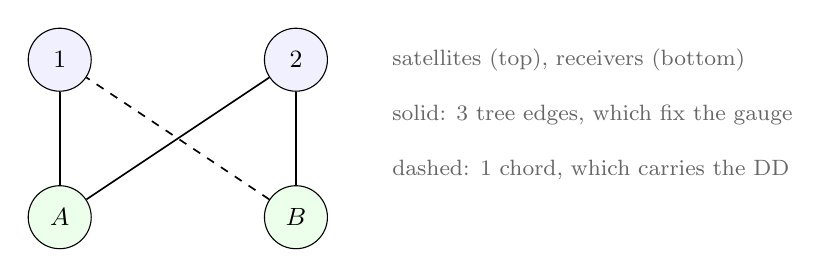
\begin{tikzpicture}[
   sat/.style={circle, draw, minimum size=8mm, inner sep=1pt, font=\small, fill=blue!6},
   rec/.style={circle, draw, minimum size=8mm, inner sep=1pt, font=\small, fill=green!8},
   tree/.style={semithick},
   chord/.style={semithick, dashed},
   lbl/.style={font=\footnotesize, text=black!60}]
  \node[sat] (s1) at (0,2)   {$1$};
  \node[sat] (s2) at (3,2)   {$2$};
  \node[rec] (rA) at (0,0)   {$A$};
  \node[rec] (rB) at (3,0)   {$B$};
  \draw[tree]  (rA) -- (s1);
  \draw[tree]  (rA) -- (s2);
  \draw[tree]  (rB) -- (s2);
  \draw[chord] (rB) -- (s1);
  \node[lbl, anchor=west] at (4.1,2.0) {satellites (top), receivers (bottom)};
  \node[lbl, anchor=west] at (4.1,1.3) {solid: 3 tree edges, which fix the gauge};
  \node[lbl, anchor=west] at (4.1,0.6) {dashed: 1 chord, which carries the DD};
\end{tikzpicture}
\caption{The smallest observation graph with a cycle: two receivers,
two satellites, four arcs.  Three arcs form a spanning tree; the fourth
is a chord, and its fundamental cycle is the one estimable double
difference \Cref{eq:carry-ex-z}.}
\label{fig:carry-ex-graph}
\end{figure}

Two exact checks of the Proposition follow.  From the truth,
$z = 5 - 3 + (-1) - 2 = -1$, an integer as required.  From the
\emph{observations} alone, with nothing estimated,
\[
(\phaseo^1_B - \phaseo^2_B) - (\phaseo^1_A - \phaseo^2_A)
  = 3.25 - 4.25 = -1,
\]
because $\beta_A$, $\beta_B$, $b^1$ and $b^2$ all cancel in the double
difference.  The carry transports this single number $-1$; every other
parameter in this subsection depends on the datum.

\paragraph{The tree pins are the datum; the chord is left free.}
Model \Cref{eq:carry-ex-model} has $2+2+4 = 8$ unknowns and $4$
observations, hence a four-dimensional null space (choose
$\delta\beta_A,\delta\beta_B,\delta b^1,\delta b^2$ freely; the
$\delta N^{\sat}_{\rx}$ follow).  Pinning the three \emph{tree}
ambiguities $N^1_A = N^2_A = N^2_B = 0$ removes three of those four
dimensions, leaving the single direction
$(\beta_A,\beta_B,b^1,b^2)\mapsto(\beta_A+t,\ \beta_B+t,\ b^1-t,\ b^2-t)$,
the one remaining receiver-versus-satellite gauge (the network's clock
gauge in miniature).  One \emph{shared} pin, $b^1 \equiv 0$, removes
it.

These four arcs contain the whole datum architecture.  The tree edges
are pinned through door~2 (locally, before the reduction), the last
gauge is fixed by the shared minimum-constraint datum, and the chord is
left free: it is the only ambiguity that carries information rather
than convention.  The pins are taken here as \emph{exact} to keep the
arithmetic simple.  The implementation realises them as tight finite
priors folded by \texttt{addStationPrior}, so the pinned columns remain
present in $\Nrr$.  The exact-pin idealisation has one visible
consequence: with the tree ambiguities identically zero, $\Czmat$ in
\Cref{eq:carry-ex-z} collapses onto the chord's own column.  With finite
pins it retains all four entries, and the fold algebra below has the
same form.

\paragraph{Arrowhead blocks.}
The shared block is ordered $\xshared = [\,b^1, b^2\,]^\Tr$ and the
free locals $\xlocal{A} = [\,\beta_A\,]$, $\xlocal{B} =
[\,\beta_B,\ N^1_B\,]^\Tr$.  With unit weights the blocks of
\dcref{eq:net-blocks}{the per-station block definitions} are
\[
\Nss^{\,A} = \bm{I}_2,\quad
\Nsr^{\,A} = \begin{bmatrix}1\\1\end{bmatrix},\quad
\Nrr^{\,A} = \begin{bmatrix}2\end{bmatrix},\quad
\bm{u}_s^{\,A} = \begin{bmatrix}3.40\\-0.85\end{bmatrix},\quad
\bm{u}_r^{\,A} = \begin{bmatrix}2.55\end{bmatrix},
\]
\[
\Nss^{\,B} = \bm{I}_2,\quad
\Nsr^{\,B} = \begin{bmatrix}1&1\\1&0\end{bmatrix},\quad
\Nrr^{\,B} = \begin{bmatrix}2&1\\1&1\end{bmatrix},\quad
\bm{u}_s^{\,B} = \begin{bmatrix}4.90\\1.65\end{bmatrix},\quad
\bm{u}_r^{\,B} = \begin{bmatrix}6.55\\4.90\end{bmatrix},
\]
with $(\Nrr^{\,B})^{-1} = \left[\begin{smallmatrix}1&-1\\-1&2
\end{smallmatrix}\right]$.  There is no $A$--$B$ block: the stations
share only $b^1$ and $b^2$.

\paragraph{Schur reduction.}
Eliminating each station's locals through
\dcref{eq:net-schur-N}{the reduced-normals equation} gives
\[
\Nss^{\,A} - \Nsr^{\,A}(\Nrr^{\,A})^{-1}\Nsr^{\,A\Tr}
  = \begin{bmatrix}\phantom{-}0.5 & -0.5\\ -0.5 & \phantom{-}0.5\end{bmatrix},
\qquad
\bm{u}_s^{\,A} - \Nsr^{\,A}(\Nrr^{\,A})^{-1}\bm{u}_r^{\,A}
  = \begin{bmatrix}\phantom{-}2.125\\ -2.125\end{bmatrix},
\]
while station $B$ contributes exactly zero to both: it has two
observations and two free locals, so eliminating the locals absorbs its
rows entirely.  Summing,
\begin{equation}
\redNss = \begin{bmatrix}\phantom{-}0.5 & -0.5\\ -0.5 & \phantom{-}0.5\end{bmatrix},
\qquad
\redus = \begin{bmatrix}\phantom{-}2.125\\ -2.125\end{bmatrix},
\qquad
\mathrm{eig}(\redNss) = \{0,\,1\}.
\label{eq:carry-ex-reduced}
\end{equation}
The reduced system has rank $1$ and one zero eigenvalue, with
eigenvector $[1,1]^\Tr$: the single gauge predicted above.  A
null-space rank gate that declares dimension $1$ for this configuration
passes; one that declares $0$ or $2$ throws
(\dcref{sec:net-sbasis}{the minimum-constraint datum section}).

\paragraph{Datum, solve, back-substitute.}
Applying the shared pin $b^1 \equiv 0$ to
\Cref{eq:carry-ex-reduced} and solving gives $\hat b^2 = -4.25$, and
back-substituting through
\dcref{eq:net-backsub}{the back-substitution equation},
\[
\hat\beta_A = 3.40,
\qquad
\hat\beta_B = 5.90,
\qquad
\hat N^1_B = -1.00 .
\]
The fit is exact (all four residuals vanish), and the result agrees to
machine precision with a dense stacked solve of the same system: the
lossless-marginalisation claim of \dcref{sec:net-schur}{the Schur
reduction section} in numbers.

These estimates do not resemble the truth.  The estimated satellite
phase bias $\hat b^2 = -4.25$ differs from $b^2 = -0.15$, and
$\hat N^1_B = -1$ differs from $N^1_B = 5$; each has absorbed the
datum.  The chord's double difference in this frame is
\[
\hat z = \hat N^1_B - \hat N^1_A + \hat N^2_A - \hat N^2_B
       = -1 - 0 + 0 - 0 = -1,
\]
identical to the truth and to the value read directly off the
observations.  Datum invariance here is an identity, not an asymptotic
property.

\paragraph{Folding a carried DD.}
Suppose the previous epoch carried this chord.  With
$\Czmat = [\,0\ \ 1\,]$ on station $B$ (one row, the exact-pin
collapse noted above), \Cref{eq:carry-fold-blocks} gives
\[
\Bfold = 2,
\qquad
\Gfold = \begin{bmatrix}\phantom{-}1\\-1\end{bmatrix},
\qquad
\zfreev = 3.25 ,
\]
and the identity $z = \zfreev - \Gfold^\Tr\xshared = 3.25 - 4.25 = -1$
recovers the DD: $\zfreev$ is a data-only quantity in the correction
frame, not the DD itself.  Also $\Gfold^\Tr[1,1]^\Tr = 0$: the fold
direction is orthogonal to the gauge, as the second Remark of
\Cref{sec:net-carry-doors} requires, so no choice of prior can make
this carry fix the datum.

\emph{A consistent carry is a no-op.}  With $\hat z = -1$ and a rigid
prior $\Pzmat = 0$, \Cref{eq:carry-fold-N,eq:carry-fold-u} reproduce
$\hat b^2 = -4.25$, $\hat\beta_A = 3.40$, $\hat\beta_B = 5.90$,
$\hat N^1_B = -1$ and zero residuals.  The innovation is
$v = 3.25 - 4.25 - (-1) = 0$.  Carrying information the data already
implies changes nothing.

\emph{A stale carry distorts the whole solution.}  Suppose instead that
the chord slipped by one cycle undetected, so $\hat z = 0$ is folded
rigidly.  Re-solving gives
\begin{center}
\begin{tabular}{@{}lccc@{}}
\toprule
 & $\hat b^2$ & $\hat\beta_A$ & $\hat\beta_B$ \\
\midrule
consistent carry ($\hat z = -1$) & $-4.25$ & $3.40$ & $5.90$ \\
stale carry ($\hat z = 0$)       & $-3.75$ & $3.15$ & $5.15$ \\
\bottomrule
\end{tabular}
\end{center}
and post-fit residuals of $+0.25$, $-0.25$, $-0.25$, $+0.25$ cycles on
rows $(A,1)$, $(A,2)$, $(B,1)$, $(B,2)$ respectively.  The one-cycle
error in a stiff carried quantity does not stay in the ambiguity that
slipped.  It moves the \emph{emitted satellite phase bias} by half a
cycle and spreads the remainder evenly over every observation in the
network.  This is the general mechanism by which a stale zero-$q$ carry
damages a solution: the network cannot reject information asserted
with infinite confidence, so it redistributes the contradiction into
whatever states can absorb it.  It is the reason for standing
invariant~1 of the project: any zero-$q$ time link requires a wired,
tested slip response before it may be armed.  Invariant~7 applies the
same reasoning to the edges of the carry: the driver treats a slipped
or unresolvable arc as a decoupling event (the chord is dropped or born
fresh, and counted), and a returning arc re-couples only through a
fresh tap-off.

\emph{The innovation test, and its limits.}  From
\Cref{eq:carry-innov}, with $\Sigss = \mathrm{diag}(0,\,1)$ (the pinned
column treated as exact),
\[
v = 3.25 - 3.75 - 0 = -0.5,
\qquad
\mathrm{Cov}(v) = \Mfold^{-1} - \Gfold^\Tr\Sigss\Gfold = 2 - 1 = 1,
\qquad
\frac{|v|}{\sqrt{\mathrm{Cov}(v)}} = 0.5 .
\]
The test detects the slip at only $0.5\sigma$, far below any usable
flag threshold (the default \texttt{network.carry\_invariant\_innov\_k}
is 4.0).  The residuals show why: with four observations and almost no
redundancy, the parameters absorbed half the error, so only half of it
reached the innovation.  The statistic is exact rather than
conservative; its \emph{power} is a property of the network's
redundancy, and a two-by-two network has almost none.  Any
estimation-side slip test is diagnostic of the carry only in proportion
to the part of the error the network cannot absorb.

\paragraph{A tree-edge death: the unimodular pivot.}
The two-by-two network is too small to show a pivot: with one chord,
every tree edge whose death matters is a cut edge.  A third satellite
gives $n_c = 2$, $m_c = 3$, $|\arcset_c| = 6$, so the tree has four
edges and there are $K_c = 2$ chords.  The tree
$\{(A,1),(A,2),(A,3),(B,1)\}$ with chords $(B,2)$ and $(B,3)$ gives
\[
z_1 = N^2_B - N^2_A + N^1_A - N^1_B,
\qquad
z_2 = N^3_B - N^3_A + N^1_A - N^1_B .
\]
Let the tree edge $(A,1)$ die.  Both chords cover it, so one covering
chord, $(B,2)$, is promoted into the tree and the dead arc is killed as
a chord.  Against the new tree
$\{(A,2),(A,3),(B,1),(B,2)\}$ the cycle basis is
\[
z_1' = N^1_A - N^1_B + N^2_B - N^2_A = z_1,
\qquad
z_2' = N^3_B - N^3_A + N^2_A - N^2_B = z_2 - z_1,
\]
that is $\bm{z}' = \bm{T}\bm{z}$ with
\[
\bm{T} = \begin{bmatrix}\phantom{-}1 & 0\\ -1 & 1\end{bmatrix},
\qquad \det\bm{T} = 1 .
\]
$\bm{T}$ is integer with unit determinant, so
$\Pzmat{}' = \bm{T}\Pzmat\bm{T}^\Tr$ is an exact change of basis: the
carried covariance is transformed without approximation.  Killing the
dead arc's row of $\bm{z}'$ is then a marginalisation, and the
surviving $z_2'$ continues with no loss.  A carry of the raw ambiguities
would require an S-transformation of a datum-dependent state for the
same graph event; the cycle basis removes that requirement.

% ------------------------------------------------------------------
\subsection{Where each object lives}
\label{sec:net-carry-map}

\begin{center}\small
\begin{tabular}{@{}p{0.30\linewidth}p{0.30\linewidth}p{0.34\linewidth}@{}}
\toprule
Object & Symbol & Home \\
\midrule
Arrowhead accumulation, Schur reduction, back-substitution &
  \texttt{addStation}, \texttt{reduce}, \texttt{reconstructStation} &
  \texttt{filter/Network\-Normal\-Equations} \\
Door 1: shared border prior &
  \texttt{addSharedInfo}, \texttt{addSharedPriorDense} &
  \texttt{filter/Network\-Normal\-Equations}, \texttt{filter/Network\-Estimator} \\
Door 2: pre-reduce local prior &
  \texttt{addStationPrior} &
  \texttt{filter/Network\-Normal\-Equations} \\
Door 3: post-reduce Woodbury folds &
  \texttt{foldReducedSumZeroGauges}, \texttt{foldReducedDdPriors} &
  \texttt{filter/Network\-Normal\-Equations} \\
Cycle algebra, lifecycle operations &
  \texttt{ArcKey}, \texttt{ZComponent} &
  \texttt{filter/NetworkZStore} \\
Per-epoch reconcile $\bm{W}$, posterior install, innovation gate &
  \texttt{buildDdPriors}, \texttt{installPosterior} &
  \texttt{filter/Network\-Invariant\-Carry\-Driver} \\
Posterior and innovation readouts &
  \texttt{ddPriorPosteriorMean}, \texttt{ddPriorPosteriorCovariance},
  \texttt{ddPriorInnovation} &
  \texttt{filter/Network\-Normal\-Equations} \\
PD screen telemetry &
  \texttt{DdFoldStats}, \texttt{ddPriorBlockDegenerate} &
  \texttt{filter/Network\-Normal\-Equations} \\
Datum and rank gate &
  \texttt{NetworkSbasis}, \texttt{assertNullSpaceRank} &
  \texttt{filter/NetworkSbasis} \\
\bottomrule
\end{tabular}
\end{center}

\ifSubfilesClassLoaded{\printbibliography}{}
\end{document}
